\documentclass[tikz, border=10pt]{standalone}
\usepackage{tikz}
\usepackage{amsmath}
\usetikzlibrary{shapes, calc, backgrounds, arrows.meta}

\begin{document}
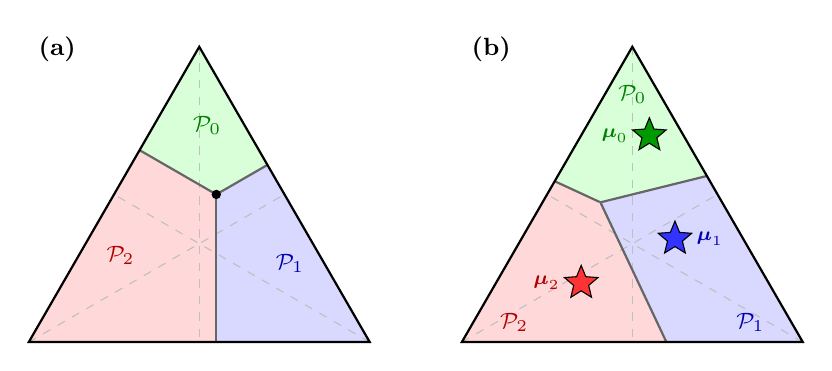
\begin{tikzpicture}[font=\sffamily]

    \begin{scope}[xshift=0.0cm, scale=0.5]
    \node[font=\small\bfseries, anchor=north west] at (-4.330, 5.500) {(a)};
    \coordinate (Top) at (0.000, 5.000);
    \coordinate (Right) at (4.330, -2.500);
    \coordinate (Left) at (-4.330, -2.500);

    \coordinate (Int) at (0.433, 1.250);

    \fill[green!15] (0.000, 5.000) -- (1.732, 2.000) -- (0.433, 1.250) -- (-1.516, 2.375) -- cycle;
    \fill[blue!15] (4.330, -2.500) -- (0.433, -2.500) -- (0.433, 1.250) -- (1.732, 2.000) -- cycle;
    \fill[red!15] (-4.330, -2.500) -- (-1.516, 2.375) -- (0.433, 1.250) -- (0.433, -2.500) -- cycle;

    \draw[dashed, gray!50, thin] (Left) -- (2.165, 1.250);
    \draw[dashed, gray!50, thin] (Right) -- (-2.165, 1.250);
    \draw[dashed, gray!50, thin] (Top) -- (0.000, -2.500);

    \draw[thick, black!60] (Int) -- (1.732, 2.000);
    \draw[thick, black!60] (Int) -- (-1.516, 2.375);
    \draw[thick, black!60] (Int) -- (0.433, -2.500);

    \node[circle, fill=black, inner sep=1.2pt] at (Int) {};

    \draw[thick] (Top) -- (Right) -- (Left) -- cycle;

    \node[green!50!black, font=\footnotesize\bfseries] at (0.200, 3.000) {$\mathcal{P}_0$};
    \node[blue!70!black, font=\footnotesize\bfseries] at (2.300, -0.500) {$\mathcal{P}_1$};
    \node[red!70!black, font=\footnotesize\bfseries] at (-2.000, -0.300) {$\mathcal{P}_2$};

    \end{scope}

    \begin{scope}[xshift=5.5cm, scale=0.5]
    \node[font=\small\bfseries, anchor=north west] at (-4.330, 5.500) {(b)};
    \coordinate (Top) at (0.000, 5.000);
    \coordinate (Right) at (4.330, -2.500);
    \coordinate (Left) at (-4.330, -2.500);

    \coordinate (Mu0) at (0.433, 2.750);
    \coordinate (Mu1) at (1.083, 0.125);
    \coordinate (Mu2) at (-1.299, -1.000);

    % Region 0 (Green)
    \begin{scope}
        \clip (Top) -- (Right) -- (Left) -- cycle;
        \path (Mu0) -- (Mu1) coordinate[midway] (M01);
        \clip ($(M01)!20cm!90:(Mu1)$) -- ($(M01)!20cm!-90:(Mu1)$) -- ($(M01)!20cm!180:(Mu1)$) -- cycle;
        \path (Mu0) -- (Mu2) coordinate[midway] (M02);
        \clip ($(M02)!20cm!90:(Mu2)$) -- ($(M02)!20cm!-90:(Mu2)$) -- ($(M02)!20cm!180:(Mu2)$) -- cycle;
        \fill[green!15] (-6,-6) rectangle (6,6);
    \end{scope}

    % Region 1 (Blue)
    \begin{scope}
        \clip (Top) -- (Right) -- (Left) -- cycle;
        \path (Mu1) -- (Mu0) coordinate[midway] (M10);
        \clip ($(M10)!20cm!90:(Mu0)$) -- ($(M10)!20cm!-90:(Mu0)$) -- ($(M10)!20cm!180:(Mu0)$) -- cycle;
        \path (Mu1) -- (Mu2) coordinate[midway] (M12);
        \clip ($(M12)!20cm!90:(Mu2)$) -- ($(M12)!20cm!-90:(Mu2)$) -- ($(M12)!20cm!180:(Mu2)$) -- cycle;
        \fill[blue!15] (-6,-6) rectangle (6,6);
    \end{scope}

    % Region 2 (Red)
    \begin{scope}
        \clip (Top) -- (Right) -- (Left) -- cycle;
        \path (Mu2) -- (Mu0) coordinate[midway] (M20);
        \clip ($(M20)!20cm!90:(Mu0)$) -- ($(M20)!20cm!-90:(Mu0)$) -- ($(M20)!20cm!180:(Mu0)$) -- cycle;
        \path (Mu2) -- (Mu1) coordinate[midway] (M21);
        \clip ($(M21)!20cm!90:(Mu1)$) -- ($(M21)!20cm!-90:(Mu1)$) -- ($(M21)!20cm!180:(Mu1)$) -- cycle;
        \fill[red!15] (-6,-6) rectangle (6,6);
    \end{scope}

    \draw[dashed, gray!50, thin] (Left) -- (2.165, 1.250);
    \draw[dashed, gray!50, thin] (Right) -- (-2.165, 1.250);
    \draw[dashed, gray!50, thin] (Top) -- (0.000, -2.500);

    \begin{scope}
        \clip (Top) -- (Right) -- (Left) -- cycle;
        \path (Mu0) -- (Mu2) coordinate[midway] (Mc02);
        \clip ($(Mc02)!20cm!90:(Mu2)$) -- ($(Mc02)!20cm!-90:(Mu2)$) -- ($(Mc02)!20cm!180:(Mu2)$) -- cycle;
        \path (Mu0) -- (Mu1) coordinate[midway] (Mb01);
        \draw[thick, black!60] ($(Mb01)!20cm!90:(Mu1)$) -- ($(Mb01)!20cm!-90:(Mu1)$);
    \end{scope}
    \begin{scope}
        \clip (Top) -- (Right) -- (Left) -- cycle;
        \path (Mu0) -- (Mu1) coordinate[midway] (Mc01);
        \clip ($(Mc01)!20cm!90:(Mu1)$) -- ($(Mc01)!20cm!-90:(Mu1)$) -- ($(Mc01)!20cm!180:(Mu1)$) -- cycle;
        \path (Mu0) -- (Mu2) coordinate[midway] (Mb02);
        \draw[thick, black!60] ($(Mb02)!20cm!90:(Mu2)$) -- ($(Mb02)!20cm!-90:(Mu2)$);
    \end{scope}
    \begin{scope}
        \clip (Top) -- (Right) -- (Left) -- cycle;
        \path (Mu1) -- (Mu0) coordinate[midway] (Mc10);
        \clip ($(Mc10)!20cm!90:(Mu0)$) -- ($(Mc10)!20cm!-90:(Mu0)$) -- ($(Mc10)!20cm!180:(Mu0)$) -- cycle;
        \path (Mu1) -- (Mu2) coordinate[midway] (Mb12);
        \draw[thick, black!60] ($(Mb12)!20cm!90:(Mu2)$) -- ($(Mb12)!20cm!-90:(Mu2)$);
    \end{scope}

    \draw[thick] (Top) -- (Right) -- (Left) -- cycle;

    \node[star, star points=5, star point ratio=2.25, fill=green!60!black, draw=black, inner sep=2pt] at (Mu0) {};
    \node[font=\scriptsize, green!50!black, anchor=east] at ($(Mu0)+(-0.300,0.000)$) {$\boldsymbol{\mu}_0$};
    \node[star, star points=5, star point ratio=2.25, fill=blue!80, draw=black, inner sep=2pt] at (Mu1) {};
    \node[font=\scriptsize, blue!70!black, anchor=west] at ($(Mu1)+(0.300,0.000)$) {$\boldsymbol{\mu}_1$};
    \node[star, star points=5, star point ratio=2.25, fill=red!80, draw=black, inner sep=2pt] at (Mu2) {};
    \node[font=\scriptsize, red!70!black, anchor=east] at ($(Mu2)+(-0.300,0.000)$) {$\boldsymbol{\mu}_2$};

    \node[green!50!black, font=\footnotesize\bfseries] at (0.000, 3.800) {$\mathcal{P}_0$};
    \node[blue!70!black, font=\footnotesize\bfseries] at (3.000, -2.000) {$\mathcal{P}_1$};
    \node[red!70!black, font=\footnotesize\bfseries] at (-3.000, -2.000) {$\mathcal{P}_2$};

    \end{scope}

\end{tikzpicture}
\end{document}
